\documentclass{beamer}
\usepackage{amsmath, amssymb, amsthm, bbm}

\usepackage{tikz}
\usepackage{tkz-berge}
\usetikzlibrary{positioning}
\usepackage[position=top]{subfig}
\usetikzlibrary{arrows, positioning, automata}

%\theoremstyle{definition}
%\newtheorem{definition}{Definition}[section]


\usepackage[utf8]{inputenc}
\usetheme{Berlin}
\title[]{Reconstruction parcimonieuse des signaux}
 
%\subtitle{The Erd\H{o}s-R\'enyi model}
 
\author[Leo Davy]{Leo Davy}
\institute{Universit\'e de Montpellier} 
\date[]{Montpellier, 1 Juin 2021}

\begin{document}

	\frame{\titlepage}

	\begin{frame}
		\frametitle{Signaux}
		\begin{columns}[T]
			\begin{column}{.65\textwidth}
				\begin{figure}
					\includegraphics[width=\textwidth]{Figs/ecg}
				\end{figure}
				\uncover<2>{
					\begin{definition}
						Un signal est une application $f:X\to Y$
					\end{definition}
				}	
			\end{column}		
			\begin{column}{.3\textwidth}
				\begin{figure}
					\includegraphics[width=\textwidth]{Figs/castle}
				\end{figure}
				\uncover<2->{
					\begin{example}[familles de signaux]
						\begin{itemize} 
							\item $\mathbb{R}^N$ 
							\item $L^2(\mathbb{R})$
						\end{itemize}
					\end{example}
				}
			\end{column}
		\end{columns}
	\end{frame}

	\begin{frame}
		\frametitle{Exemples de problèmes}
		\begin{columns}[T]
			\begin{column}{.35\textwidth}
				\begin{itemize}
					\item Compresser un signal
					\item Décomposer un signal en éléments simples
					\item Reconstruire un signal en utilisant un minimum de mesures
				\end{itemize}
			\end{column}
			\begin{column}{.6\textwidth}
				\includegraphics[width=.7\textwidth]{Figs/castle_wavelet}
				TODO: ajouter image fourier-dirac+fourier sous-échantilloné
			\end{column}
		\end{columns}
	\end{frame}


	\begin{frame}
		\frametitle{Traitement du signal}
		\begin{columns}[T]
			\begin{column}{.4\textwidth}
				\begin{block}{Mesure du signal}
					Opérateur d'analyse
					\begin{equation*}
						A:f\mapsto (c_i(f))_I
					\end{equation*}
					avec $c_i(f) = \langle f, \varphi_i \rangle$.
				\end{block}
				\uncover<2->{
					\begin{block}{Reconstruction}
						Opérateur de synthèse
						\begin{equation*}
							S:(c_i(f))_I \mapsto f
						\end{equation*}
					\end{block}
				}
			\end{column}

			\begin{column}{.6\textwidth}
				\includegraphics[width=.95\textwidth]{Figs/scal_prod}\newline
				\uncover<2->{
					\includegraphics[width=.45\textwidth]{Figs/dirac_sparse}
					\includegraphics[width=.45\textwidth]{Figs/dirfour}
				}
				\uncover<3->{
					Quelles conditions pour reconstruire n'importe quel signal $f$ de $\mathcal{F}$ à partir de $A(f)$ ?
				}
			\end{column}
		\end{columns}	
	\end{frame}
	\begin{frame}
		\frametitle{Théorie des frames}
		\begin{columns}[T]
			\begin{column}{.7\textwidth}

				\begin{definition}
					On appelle $F = (\varphi_i)_I$ un frame de $H$ si $\exists m, M >0$ tels que
					\begin{equation*}
						m||f||_2^2 \leq \sum_I |\langle f, \varphi_i \rangle |^2 \leq M ||f||_2^2, \quad \forall f \in H
					\end{equation*}
				\end{definition}
			\end{column}
			\begin{column}{.25\textwidth}
				\includegraphics[width=1.1\textwidth]{Figs/frameR2}
			\end{column}
		\end{columns}
		\uncover<2->{ 
			\begin{block}{Frame serré}
				Si $m=M$, formule de reconstruction :
				\begin{equation*}
					f = \frac{1}{M} \sum_I \langle f, f_i \rangle f_i. 
				\end{equation*}
			\end{block}
		}
	\end{frame}
	\begin{frame}
		\frametitle{Décomposition en ondelettes}
		\begin{columns}[T]
			\begin{column}{.3\textwidth}
				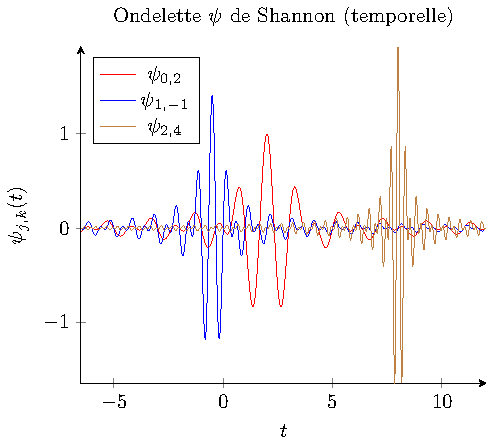
\includegraphics[width=\textwidth]{Figs/shannonspat}
				\begin{align*}
					f =&\sum_{k=-\infty}^{+\infty} \langle f, \varphi_k \rangle\varphi_k \\
					&+ \sum_{j=1}^{+\infty} \left(\sum_{k=-\infty}^{+\infty} \langle f, \psi_{j,k} \rangle \psi_{j,k}\right)
				\end{align*}
			\end{column}
			\begin{column}{.6\textwidth}
				\begin{equation*}
					\psi_{j,k} := 2^{j/2}\psi(2^j\cdot -k).
				\end{equation*}
				$j$ : échelle (fréquence), $k$ : localisation
				\includegraphics[height=.20\textheight]{Figs/mallatdisctop}
				\includegraphics[height=.46\textheight]{Figs/mallatdiscbot}
			\end{column}
		\end{columns}
	\end{frame}

	\begin{frame}
		\frametitle{Compression par les ondelettes}
		\begin{columns}[T]
			\begin{column}{.5\textwidth}
				Moments nuls : $\langle P, \psi_{j,k} \rangle = 0$ si $\deg(P)\leq m$\newline
			\uncover<3->{\underline{Jaffard 91 :} $f\in C^\alpha$ et $\psi$ avec $m\geq\alpha$ moments nuls, alors
				\begin{equation*}
					|\langle f, \psi_{j,k}\rangle| \leq C_\alpha 2^{-j(\alpha + \frac{1}{2})}
				\end{equation*}
				\includegraphics[width=.9\textwidth]{Figs/mallatcont}
				}
			\end{column}
			\begin{column}{.5\textwidth}
					\includegraphics[width=.40\textwidth]{Figs/daubechies}
					\includegraphics[width=.9\textwidth]{Figs/boatsnonlin}
			\end{column}
		\end{columns}
	\end{frame}

	\begin{frame}
		\frametitle{Une représentation parcimonieuse "optimale" ?}
		Soit $D = (\varphi_i)_I$ une famille de vecteurs (dictionnaire d'atomes), $f\in Vect(D)$ :
		\begin{enumerate}
			\item Reconstruction : Quels $(c_i)_J$ pour que $f=\sum_{J} c_i \varphi_i$ ?
			\uncover<2->{
				\item Reconstruction parcimonieuse : Quels $(c_i)_I$ minimise le nombre de coefficients non nuls et reconstruit $f$?
				}
		\end{enumerate}
		\uncover<3->{
			Problème P0 (décomposition atomique) :
			\begin{equation*}
				\min ||x||_0 : f = F_D x
			\end{equation*}
			avec $x=(c_i)_J$ et $F_D$ matrice dont les colonnes sont les $\varphi_i$.
			}
		\uncover<4->{
			Est-ce bien posé ? Est-ce calculable ?
			}
	\end{frame}

	\begin{frame}
		\begin{example}[Fourier-Dirac]
			$D = (T, W)$ avec $T=(\delta_k)_{0\leq k \leq N-1}$ et $W=(\frac{e^{-\frac{2i\pi k\cdot}{N}}}{\sqrt{N}})_{0\leq k\leq N-1}$
		\end{example}
		\begin{theorem}[Donoho-Stark 89]
			Soit $f\in\mathbb{R}^N$ un signal non nul, alors
			\begin{equation}
				||F_T f||_0 + ||F_W f||_0 \geq 2\sqrt{N}
			\end{equation}
		\end{theorem}
		\begin{theorem}[Donoho-Stark 89]
			Soit $f\in\mathbb{R}^N$ et $x=(x_T, x_W)$ tel que $f = F_T x_T + F_W x_W$ et $||x||_0<\sqrt{N}$.
			Alors $x$ est l'unique solution de P0.
		\end{theorem}
	\end{frame}

	\begin{frame}
		Principe d'incertitude $\rightarrow$ Unicité de la décomposition atomique\newline
		Cas particulier du dictionnaire Fourier-Dirac ?
		\uncover<2->{
			Non, la matrice clef dans la preuve est  :
			\begin{equation*}
				F_{W}^tF_{T} = 
				\begin{bmatrix}
			\langle \psi_1, \varphi_1 \rangle & 	\langle \psi_1, \varphi_2 \rangle	&\cdots 	&	\langle \psi_1, \varphi_N \rangle\\
			\langle \psi_2, \varphi_1 \rangle & 	\ddots 					& \vdots 	&	\langle \psi_2, \varphi_N \rangle \\
			\vdots 				& \cdots 				&\ddots 	 	&	\vdots \\
			\langle \psi_N, \varphi_1 \rangle & \cdots 				& \cdots 		&	 \langle \psi_N, \varphi_N \rangle. 
				\end{bmatrix}
			\end{equation*}
			}
			\uncover<3->{
				Quantité clef : $M = max_{i,j} |\langle \psi_i, \varphi_j \rangle|$ (incohérence)
				}
	\end{frame}

	\begin{frame}
		Soit $D=(\Psi,\Phi)$ une paire de bases arbitraires de $\mathbb{R}^N$ et $M=max_{i,j}|\langle \psi_i, \varphi_j \rangle|$.
		\begin{theorem}[Principe d'incertitude généralisé]
			Soit $f\in\mathbb{R}^N$ un signal non nul.
			Alors
			\begin{equation*}
				||F_\Psi f||_0 + ||F_\Phi f||_0 \geq \frac{2}{M}
			\end{equation*}
		\end{theorem}
		\uncover<2->{
		\begin{theorem}[Unicité de la solution de P0 généralisé]
			Soit $f\in\mathbb{R}^N$ alors la décomposition atomique $x$ de $f$ est unique si $||x||_0<\frac{1}{M}$.
		\end{theorem}
		}
		Dictionnaire Fourier-Dirac : $M=\frac{1}{\sqrt{N}}$.
	\end{frame}

	\begin{frame}
		\begin{columns}[T]
			\begin{column}{.6\textwidth}
				P1 :
				\begin{equation}
					\min ||x||_1 : f = F_D x
				\end{equation}
				Avantages :
				\begin{enumerate}
					\item Sous des hypothèses de parcimonie, la solution de P1 coincide avec celle de P0.
					\item Beaucoup d'algorithmes efficaces de résolution (Programmation linéaire) 		
				\end{enumerate}	
			\end{column}
			\begin{column}{.4\textwidth}
				\includegraphics[width=\textwidth]{Figs/l1vsl2}
			\end{column}
		\end{columns}
	\end{frame}

	\begin{frame}
		\begin{theorem}
			Soit $D=(\Phi,\Psi)$ une paire de bases orthonormales et soit $f\in\mathbb{R}^N$ un signal, $x_0$ la solution de P0 pour $f=F_Dx$, si l'une des hypothèses suivantes est vérifiée :
			\begin{columns}[T]
				\begin{column}{.6\textwidth}
					\begin{itemize}
						\item (Donoho-Huo 98) $||x_{0,\Phi}||_0 + ||x_{0,\Psi}|| < \frac{1}{2M}$
						\uncover<2->{\item (Elad-Bruckstein 02) $||x_{0,\Phi}||_0 + ||x_{0, \Psi}||_0 < \frac{\sqrt{2} - 0.5}{M} \sim \frac{0.92}{M}$}
						\uncover<3->{\item 	$||x_{0, \Phi}||_0 < \frac{1}{2M}$ et $||x_{0, \Psi}||_0 < \frac{1}{2M}$} 
					\end{itemize}
				\end{column}
				\begin{column}{.4\textwidth}
					\includegraphics[width=.95\textwidth]{Figs/result}
				\end{column}
			\end{columns}
			alors $x_0$ est l'unique solution de P1.
		\end{theorem}
		\uncover<4->{
			Généralisations : Dictionnaire de bases arbitraire, frames (Torrésani 15).
			}
	\end{frame}

	\begin{frame}
		Comment démontrer ces théorèmes ?\newline
		Avec un principe d'incertitude.
		\uncover<2->{
			\newline 
			$\mathcal{N} = \{\delta : F_D \delta = 0\}$. On pose 
			\begin{equation}
				\mu(\Gamma_\Phi, \Gamma_\Psi) = \sup_{\delta \in \mathcal{N}} \frac{ \sum_{i\in \Gamma_\Phi} |\delta_{\Phi, i}| + \sum_{i\in\Gamma_\Psi}|\delta_{\Psi, i}|}{||\delta_\Phi||_1 + ||\delta_\Psi||_1}
			\end{equation}
			}
		\uncover<3->{
			\begin{lemma}[Donoho-Huo 98]
				Si $\mu(\Gamma_\Phi, \Gamma_\Psi) < \frac{1}{2}$ alors n'importe quelle solution de $f=F_D x$ supportée sur $\Gamma_\Phi\cup\Gamma_\Psi$ est l'unique solution de P1.
			\end{lemma}
		}
	\end{frame}

	\begin{frame}
		On sait :
		\begin{itemize}
			\item Trouver la décomposition atomique d'un signal parcimonieux 
			\uncover<5->{\item Représenter un signal régulier avec peu de coefficients (ondelettes)}
		\end{itemize}
		\uncover<3->{
			Difficultés :
			\begin{itemize}
				\item Hypothèses de parcimonie fortes
				\uncover<6->{\item Il faut faire toutes les mesures puis enlever la plupart des coefficients} 
			\end{itemize}
			}
		\uncover<4->{
			Solutions :
			\begin{itemize}
				\item \underline{Candes-Romberg 06:} Pour l'équivalence P0-P1, avec probabilité tendant vers 1, il suffit d'avoir $||x||_0 < \frac{C}{M^2\log(N)}$.
				\uncover<7->{\item \underline{Candes-Romberg 06:} Pour reconstruire un signal avec $S$ coefficients non nuls, avec probabilité tendant vers 1, il suffit de faire $S\log(N)$ mesures et résoudre P1.}  
			\end{itemize}
		}
	\end{frame}

	\begin{frame}
		\frametitle{Compressed sensing}
		\underline{Idée :} Exploiter la parcimonie pour faire moins de mesures 
		\uncover<2->{
			\begin{columns}[T]
				\begin{column}{.5\textwidth}
					Cadre du problème : $F_\Phi$ matrice d'analyse, $\Omega \subset \{0,\cdots, N-1\}$.\newline
					On mesure $y_\Omega = F_{\Phi, \Omega} s$, on veut retrouver $s$.\newline 
				\end{column}
				\begin{column}{.5\textwidth}
					\includegraphics[width=.9\textwidth]{Figs/mesure_gauss}
				\end{column}
			\end{columns}
		}

		\uncover<3->{Difficulté : système sous déterminé $K:=\mathbb{E}(|\Omega|)<<N$\newline}
		\uncover<4->{Solution : $s$ est parcimonieux dans une base}
	\end{frame}

	\begin{frame}
		P1 (Compressed Sensing):
		\begin{equation*}
			\min_{x\in\mathbb{R}^N} ||x||_1 : F_{\Phi,\Omega} x = F_{\Phi,\Omega}s
		\end{equation*}

		\begin{itemize} 
			\item Matrice gaussienne $F_{G, \Omega} = (c_{i,j})_{(i,j)\in\Omega\times \{0,\cdots, N-1\}}$ avec $c_{i,j}\sim N(0, \frac{1}{\sqrt{N}})$
			\item Matrice de Fourier $F_{F, \Omega}$ restriction aux lignes indexées par $\Omega$ de la matrice de Fourier.
		\end{itemize}
	\end{frame}

	\begin{frame}
		\frametitle{Axiomes}
		\begin{definition}
			On dit que $F_\Omega$ vérifie 
			\begin{itemize}
				\item $\lambda$-UUP si 
					\begin{equation*}
						\frac{K}{2N}||x||_2^2 \leq ||F_\Omega x||_2^2 \leq \frac{3K}{2N}||x||_2^2
					\end{equation*}
				\uncover<2->{	\item $\lambda$-ERP si, en notant $\sigma = sign(x)$, il existe $P\in\mathbb{R}^N$ tel que 
				\begin{enumerate}
					\item $P(t) = \sigma(t), \forall t \in supp(x)$
					\item $\exists Q\in\mathbb{R}^\Omega$ tel que $P=F_\Omega^*Q$
					\item $P(t) < \frac{1}{2}, \forall t \notin supp(x)$} 
				\end{enumerate}
			\end{itemize}
			est vrai avec probabilité au moins  $1-\mathcal{O}(N^{-\rho/\alpha})$ pour tout signal $x\in\mathbb{R}^N$ $S$-parcimonieux qui vérifie
			\begin{equation*}
				S \leq \alpha \frac{K}{\lambda}.
			\end{equation*}
		\end{definition}	
	\end{frame}

	\begin{frame}
		\begin{example}
			\begin{itemize}
				\item La matrice Gaussienne $F_{G, \Omega}$ vérifie $\log(N)$-UUP et $\log(N)$-ERP 
				\item La matrice de Fourier $F_{F, \Omega}$ vérifie  $\log(N)^5$-UUP et $\log(N)$-ERP
			\end{itemize}
		\end{example}
	\end{frame}

	\begin{frame}
		\begin{theorem}[Candes-Tao 04]
			Soit $F_\Omega$ qui vérifie $\lambda$-ERP et $\lambda$-UUP.
			Soit $K\geq \lambda$.
			\newline
			Soit $s$ un signal dans $\mathbb{R}^N$ tel que ses coefficients dans une base de référence décroissent comme :
			\begin{equation*}
				|\theta_{(n)}| \leq C n^{-\frac{1}{p}}
			\end{equation*}
			pour un certain $C >0$ et $0 < p \leq 1$. 
			\newline
			On pose $r = \frac{1}{p} - \frac{1}{2}$, alors n'importe quelle solution $x$ de (P1) vérifie :
			\begin{equation*}
				||s - x||_2 \leq C_r \left(\frac{K}{\lambda}\right)^{-r}
			\end{equation*}
			avec probabilité au moins $1 - \mathcal{O}(N^{-\frac{\rho}{\alpha}})$, pour certains $\rho$ et $\alpha$.
		\end{theorem}
	\end{frame}

	\begin{frame}
		\frametitle{Conséquences des théorèmes}
		TODO : ajouter image des reconstructions CS 
	\end{frame}

	\begin{frame}
		\frametitle{Conclusion}
		\begin{itemize}
			\item On peut représenter de façon parcimonieuse des signaux réguliers (ondelettes)
			\item On peut résoudre le problème de décomposition atomique (P1)	
			\item Pour reconstruire un signal $S$-parcimonieux, $S\log(N)$ mesures suffisent (Compressed sensing)
		\end{itemize}
	\end{frame}


	\begin{frame}
		\frametitle{Les ondelettes par l'analyse multi-échelle TODO:enlever}
		Si on a des sous espaces emboités
		\begin{equation*}
			\raggedleft
			\{0\} = \lim_{N\to-\infty} \bigcap_{-\infty}^N V_j \subset \cdots \subset V_{-1} \subset V_0 \subset V_1 \subset \cdots \subset \lim_{N\to\infty}\bigcup_{-\infty}^{+\infty} V_j = L^2(\mathbb{R})
		\end{equation*}
		avec $V_j = V_{j-1}\oplus W_j$,
		alors on a la formule de reconstruction :
		\begin{equation}
			f = \pi_{V_0}(f) + \sum_{k\geq 1} \pi_{W_k}(f)\quad, \forall f \in L^2(\mathbb{R}). 
		\end{equation}

	\end{frame}

	\begin{frame}
		\frametitle{TODO:enlever}
		Deux propriétés supplémentaires pour que l'analyse soit multi-échelle :
		\begin{itemize}
			\item $f \in V_0 \iff f(\cdot -k) \in V_0 \forall k \in \mathbb{Z}$.
			\item $f \in V_0 \iff f(2^j \cdot) \in V_j \forall j \in \mathbb{Z}$
		\end{itemize}
		Et les ondelettes ?
		\begin{definition}
			On note 
			\begin{equation}
				\psi_{j,k} := 2^{j/2}\psi(2^j\cdot -k).
			\end{equation}
			On appelle $\psi$ une ondelette si $(\psi_{j,k})_{j,k\in\mathbb{Z}\times\mathbb{Z}}$ est une base de $L^2(\mathbb{R})$. 
		\end{definition}
		$j$ : échelle (fréquence), $k$ : localisation

	\end{frame}

	\begin{frame}
		\frametitle{TODO:enlever}
		La famille $(\psi_{j,k})_{k\in\mathbb{Z}}$ est une base de $W_j$. De plus, on peut associer à $\psi$ une application $\varphi$ appelée ondelette d'échelle et telle que 
		$(\varphi_k)_{k\in\mathbb{Z}} = (\varphi(\cdot -k))_{k\in\mathbb{Z}}$ soit une base de $V_0$.
		\newline
		Formule de reconstruction valable sur $L^2(\mathbb{R})$.
		\begin{equation}
			f =\sum_{k=-\infty}^{+\infty} \langle f, \varphi_k \rangle\varphi_k + \sum_{j=1}^{+\infty} \left(\sum_{k=-\infty}^{+\infty} \langle f, \psi_{j,k} \rangle \psi_{j,k}\right)
		\end{equation}
	\end{frame}
	\begin{frame}
		\frametitle{Approximation rapide ?TODO:enlever}
		Mallat : $\sum_{k=0}^{+\infty} k^{2r}|\langle f, g_k \rangle|^2 \iff \varepsilon_{(g_k)}(N, f) = o(N^{-2r})$\newline
		Jaffard (91) : $f$ $\alpha$-Lipschitzienne en $t_0$ et $\psi$ a $m>\alpha$ moments nuls $\implies |\langle f, \psi_{j,k} \rangle| \leq C_\alpha 2^{-j(\alpha + \frac{1}{2})}(1+|2^{-j}k -t_0|2^{j\alpha})$
		TODO : ajouter images décroissance coeffs ondelette discret et continue
		Conséquences : JPEG2000, une représentation parcimonieuse des signaux ?
	\end{frame}


	\begin{frame}
		TODO:enlever 
		\underline{Premier cas :} On connait une base $\Psi$ telle que $s=\Psi x_0$ avec $x_0$ parcimonieux. \newline
		On prend une mesure $\Phi$ incohérente avec $\Psi$ et on cherche la solution P1 de $y=F_\Phi F_\Psi x$ (c'est $x_0$ sous des hypothèses fortes).
		\newline
		\uncover<2->{Compressed sensing : on ne fait que les mesures indéxées par $\Omega$. Quelle est la probabilité pour que la solution de P1 de $y_\Omega = F_{\Phi, \Omega} F_\Psi x$ soit différente de $x_0$ ?} 
		\uncover<3->{Faible.\newline}

		
		\underline{Second cas:} On ne sait pas dans quelle base le signal est parcimonieux. \newline
		On prend les vecteurs de $\Phi$ tirés uniformément au hasard sur $S^{N-1}$, alors la distribution de $F_\Phi$ est invariante par changement de base, donc $F_{\Phi, \Omega}$ est presque sûrement incohérente avec une base $\Psi$ arbitraire.
		\uncover<2->{\newline
		Donc pour une matrice $F_\Phi$ de ce type, la probabilité de succès ou d'échec de la reconstruction ne dépend pas de la base $\Psi$.
		}
	\end{frame}

	\begin{frame}
		\frametitle{Résoudre P0 ?}
		On sait que dans le cas d'une paire de bases incohérentes, la solution est unique si suffisamment parcimonieuse.
		\newline
		Comment obtenir une telle solution ? 
		\uncover<2->{
			En général : très difficile 
			}
		\uncover<3->{\newline
		Solution : résoudre un autre problème et exploiter la parcimonie.
		}
	\end{frame}




\end{document}	

